\chapter{Progettazione}
\label{chap:progettazione}
Una parte consistente del monte ore iniziale dello stage è stata investita nella fase di progettazione: definizione dell’architettura del modulo di previsione, individuazione dei confini funzionali e selezione degli strumenti. Le prime settimane sono state dedicate alla prova comparativa delle tecnologie (modello, API, orchestrazione), allo studio della documentazione ufficiale e alla costruzione di prototipi rapidi; ciò ha permesso di arrivare alla fase successiva con scelte già validate e di avviare lo sviluppo su basi stabili.

\section{Tecnologie e strumenti}
\label{sec:tecnologie-strumenti}
In questa sezione sono elencate le principali tecnologie e librerie adottate per lo sviluppo del modulo di previsione, con una breve descrizione delle loro funzionalità.

\subsection{Linguaggi di programmazione}
\begin{itemize}
    \item \textbf{Python}\footnote{\url{https://www.python.org/}}: linguaggio di programmazione interpretato, ad alto livello e tipizzato dinamicamente, progettato per leggibilità e rapidità di sviluppo. Offre un vasto ecosistema di librerie per calcolo scientifico, machine learning e sviluppo applicativo.
    \item \textbf{SQL}: è un linguaggio dichiarativo standardizzato per definire, interrogare e manipolare dati all’interno di database relazionali. Fornisce strumenti per creare schemi, gestire transazioni ed eseguire query complesse in modo ottimizzato. È il mezzo principale per accedere e gestire dati strutturati in sistemi informativi.
    
\end{itemize}

\subsection{Framework e server web}
\begin{itemize}
    \item \textbf{FastAPI}\footnote{\url{https://fastapi.tiangolo.com/}}: FastAPI è un framework web Python ad alte prestazioni per la creazione di API basate su standard come OpenAPI e JSON Schema. Utilizza tipizzazione Python e Pydantic per validazione automatica e autogenerazione della documentazione.
    \item \textbf{Uvicorn}: server ASGI leggero e ad alte prestazioni, basato su uvloop e httptools, progettato per applicazioni web asincrone in Python. Fornisce un runtime veloce e a bassa latenza ideale per framework come FastAPI.
\end{itemize}

\subsection{Database e ORM}
\begin{itemize}
    \item \textbf{SQLAlchemy}: toolkit SQL e ORM per Python che fornisce un livello di astrazione avanzato per interagire con database relazionali.
    \item \textbf{Alembic}\footnote{\url{https://alembic.sqlalchemy.org/}}: strumento di database migration per SQLAlchemy che gestisce in modo versionato l’evoluzione degli schemi relazionali. Permette di generare, applicare e monitorare migrazioni tramite script incrementali.
    \item \textbf{DuckDB}: è un database analitico in-process orientato alle query OLAP, progettato per esecuzioni ad alte prestazioni direttamente all’interno dell’applicazione. Utilizza un motore vettorizzato e columnar per elaborare rapidamente grandi dataset senza necessità di un server esterno.
    \item \textbf{ChromaDB}: database vettoriale progettato per l’indicizzazione e la ricerca semantica tramite embedding ad alta dimensionalità. Fornisce storage ottimizzato, funzioni di similarity search e gestione di metadata per applicazioni LLM e retrieval-augmented.
\end{itemize}

\subsection{Autenticazione e sicurezza}
\begin{itemize}
    \item \textbf{PyJWT}\footnote{\url{https://pyjwt.readthedocs.io/}}: libreria Python per creare, firmare e validare JSON Web Token (JWT), utilizzati per autenticazione e scambio sicuro di informazioni.
\end{itemize}

\subsection{Machine Learning e Data Science}
\begin{itemize}
    \item \textbf{Pydantic}\footnote{\url{https://pydantic.dev/}}: libreria Python per la validazione e la gestione di dati basata su annotazioni di tipo. Consente di definire modelli di dati con tipi forti, validazione automatica e serializzazione/deserializzazione in modo semplice ed efficiente.
    \item \textbf{Pandas}: libreria Python per la manipolazione e l’analisi di dati strutturati, basata su oggetti fondamentali come DataFrame e Series. Offre strumenti ad alte prestazioni per filtrare, trasformare, aggregare e pulire dataset.
    \item \textbf{NumPy}: libreria Python per il calcolo scientifico che fornisce array n-dimensionali ad alte prestazioni e operazioni vettorializzate. Include funzioni per algebra lineare, statistica e trasformazioni numeriche ottimizzate in C.
    \item \textbf{scikit-learn}: libreria Python per il machine learning che offre algoritmi efficienti per classificazione, regressione, clustering e riduzione della dimensionalità. Fornisce API uniformi, strumenti per preprocessing, valutazione dei modelli e pipeline.
    \item \textbf{XGBoost}\footnote{\url{https://xgboost.ai/}}: libreria Python ottimizzata per gradient boosting che implementa alberi decisionali ad alte prestazioni, pensata per competizioni di machine learning e applicazioni industriali. Utilizza parallelismo, pruning avanzato e ottimizzazioni su memoria e GPU. È nota per l’elevata accuratezza e l’efficienza su grandi dataset tabulari.
    \item \textbf{SHAP}\footnote{\url{https://shap.readthedocs.io/}}: libreria Python che fornisce metodi basati sui valori di Shapley per interpretare modelli di machine learning. Calcola contributi locali e globali delle feature alle predizioni. È ampiamente utilizzata per garantire trasparenza, explainability e analisi di modelli complessi come XGBoost
\end{itemize}

\subsection{Strumenti di testing e deployment}
\begin{itemize}
    \item \textbf{Pytest}: framework di testing per Python che permette di scrivere test semplici, modulari e scalabili tramite un approccio basato su funzioni e fixture. Supporta parametric testing, plugin estendibili e rilevamento automatico dei test.
    \item \textbf{Docker}\footnote{\url{https://www.docker.com/}}: piattaforma di containerizzazione che consente di impacchettare applicazioni e dipendenze in ambienti isolati e portabili chiamati container. Utilizza un motore leggero basato su immagini stratificate per garantire coerenza tra ambienti di sviluppo, test e produzione. Facilita il deployment scalabile e riproducibile di applicazioni moderne.
\end{itemize}

\section{Architettura}
\label{sec:architettura}

L’architettura complessiva del sistema (Figura~\ref{fig:architettura-generale}) è stata progettata secondo principi di modularità e componibilità, in modo da permettere l’evoluzione indipendente dei singoli blocchi funzionali. 
Il modulo \textit{ErpAI-Forecasting} si inserisce come componente aggiuntivo della piattaforma ErpAI e fornisce funzionalità di previsione basate su modelli di machine learning. 
Tutte le comunicazioni verso il modulo avvengono tramite l’API Gateway, che gestisce la validazione dei token JWT presso l’Auth Server, l’instradamento delle richieste e l’esposizione controllata delle API pubbliche e interne.

L’orchestrazione vera e propria è realizzata all’interno del Modulo di Previsione, che combina tre elementi chiave: dati ERP sincronizzati tramite DuckDB, un modello XGBoost ottimizzato per il dominio applicativo, e un sistema di persistenza distribuito che comprende Prevision DB e Chroma DB. 
Questa architettura permette di separare nettamente l’elaborazione analitica (DuckDB), l’inferenza e l’explainability (Modulo di Previsione) e la persistenza (Prevision DB / Chroma DB).  
La presenza di contratti ben definiti (schema delle API REST, modelli Pydantic, formati dei dataset e versioning dei modelli) garantisce la possibilità di sostituire o aggiornare ciascun componente senza introdurre impatti a catena sugli altri servizi.

\begin{figure}[H]
    \centering
    \makebox[\textwidth][c]{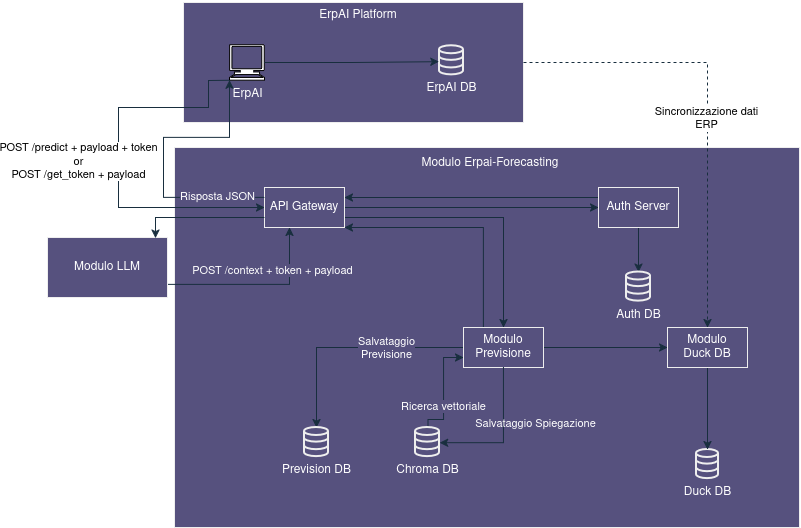
\includegraphics[width=1.1\linewidth]{img/Architettura_1.png}}
    \caption{Architettura complessiva del modulo ErpAI-Forecasting}
    \label{fig:architettura-generale}
\end{figure}

\subsection{API Gateway}
Il sistema utilizza Kong\footnote{\url{https://konghq.com/}} come API Gateway per garantire un unico punto di ingresso alle API esposte dal modulo \textit{ErpAI-Forecasting}.  
Kong gestisce instradamento, rate limiting, logging e policy di sicurezza, consentendo di centralizzare funzioni trasversali che altrimenti dovrebbero essere replicate nei singoli servizi.  
Ogni richiesta proveniente da ErpAI o dal Modulo LLM viene validata e inoltrata al Modulo di Previsione solo dopo la verifica del token JWT.

\subsection{Auth Server}
L’Auth Server è responsabile dell’autenticazione e dell’emissione dei token JWT.  
Espone endpoint per la richiesta di credenziali, la validazione dei token e la gestione di client applicativi autorizzati.  
Si appoggia ad Auth DB per memorizzare utenti, ruoli e chiavi pubbliche/privati necessarie alla firma e alla verifica dei token.  
L’API Gateway consulta l’Auth Server (o i suoi metadati JWKS) per validare l’autenticità delle richieste in ingresso.

\subsection{Modulo DuckDB}
DuckDB è il database embedded che alimenta il forecasting e ospita la replica dei dati ERP. La configurazione legge l’URL da \texttt{DUCKDB\_URL} (o \texttt{DUCKDB\_DATABASE\_URL} nel servizio di sync), costruisce il percorso su filesystem e, se la directory non è scrivibile, ripiega su un file locale in sola lettura quando già esistente. Il repository di forecasting espone \texttt{fetch\_fact\_invoices}, che restituisce \texttt{fact\_invoices} come DataFrame Pandas da usare per normalizzazione e preparazione dei dataset.
\begin{itemize}
    \item \textbf{Sincronizzazione}: un servizio di orchestrazione preleva i dati ERP attraverso i seguenti metodi:
    \begin{itemize}
        \item \textbf{fetch\_invoices}: sincronizza la tabella \texttt{invoices} con le informazioni delle fatture di vendita emesse.
        \item \textbf{fetch\_articles}: sincronizza la tabella \texttt{articles} con tutti gli articoli in vendita.
        \item \textbf{fetch\_customers}: sincronizza la tabella \texttt{customers} con l’anagrafica clienti.
        \item \textbf{fetch\_vat\_options}: sincronizza la tabella \texttt{vat\_options} con le aliquote IVA.
        \item \textbf{fetch\_article\_invoice}: sincronizza la tabella \texttt{article\_invoice} con le righe degli articoli presenti nelle fatture.
    \end{itemize}
    \item \textbf{Costruzione di \texttt{fact\_invoices}}: dopo la sincronizzazione viene ricreata la tabella \texttt{fact\_invoices}, che aggrega le informazioni rilevanti per il forecasting calcolando metriche come il totale fatturato per cliente, articolo e periodo.
\end{itemize}

\subsection{Modulo di Previsione}
Il Modulo di Previsione orchestrato da FastAPI gestisce l’intero ciclo di inferenza, dall’accesso ai dati fino alla persistenza dei risultati. Gli endpoint REST validano il payload (Pydantic), avviano un job tracciato e coordinano i servizi sottostanti:
\begin{itemize}
    \item \textbf{Acquisizione dati}: lettura delle \texttt{fact\_invoices} da DuckDB, normalizzazione di colonne/tempi e copertura mensile per articolo; filtri opzionali sulla data di cutoff.
    \item \textbf{Feature engineering}: costruzione del dataframe utilizzato per il training del modello e aggiunta di feature derivate come lag, rolling, trend stagionali e indicatori temporali.
    \item \textbf{Inferenza XGBoost}: allenamento del modello XGBoost sui dati raccolti e generazione delle previsioni per il periodo richiesto con calcolo delle metriche di accuratezza come MAPE, WAPE e RMSE.
    \item \textbf{Spiegazioni SHAP}: calcolo dei valori SHAP per ogni previsione generata, con estrazione delle feature più influenti.
    \item \textbf{Persistenza}: i risulrttati numerici, le spiegazioni e le metriche vengono salvati in Prevision DB e Chroma DB per consentire consultazioni future e audit dei processi.
    \item \textbf{Notifiche e callback}: al termine del job di previsione viene inviata una notifica di completamento ad ErpAI tramite callback HTTP, includendo lo stato e i riferimenti ai risultati salvati.
\end{itemize}

\subsection{Prevision DB}
Prevision DB conserva job, run di previsione e righe di output. Le principali tabelle sono:
\begin{itemize}
    \item \textbf{jobs}: contiene i job di previsione ed è composta da:
    \begin{itemize}
        \item \textbf{id}: identificativo univoco del job.
        \item \textbf{status}: stato del job (in coda, in esecuzione, completato, fallito).
        \item \textbf{detail}: dettaglio/errore se presente.
        \item \textbf{dataset\_id}: riferimento al dataset sincronizzato usato dal job.
        \item \textbf{timestamp}: creazione, avvio, fine ed ultimo aggiornamento.
    \end{itemize}
    \item \textbf{forecast\_runs}: registra le esecuzioni di previsione, con:
    \begin{itemize}
        \item \textbf{id}: identificativo del run.
        \item \textbf{mape}: metrica di errore della previsione usata per valutare la run.
        \item \textbf{created\_at}: data e ora di creazione della run.
    \end{itemize}
    \item \textbf{predictions\_xgboost}: contiene le righe previsionali, con:
    \begin{itemize}
        \item \textbf{forecast\_id}: riferimento alla run che ha generato la previsione.
        \item \textbf{article\_id} e \textbf{article\_name}: articolo a cui si riferisce la previsione.
        \item \textbf{prediction\_date}: data della previsione.
        \item \textbf{predicted\_quantity}: quantità stimata.
    \end{itemize}
\end{itemize}
La struttura dei dati consente di collegare job, run e singole previsioni, supportando consultazioni e analisi successive.

\subsection{Chroma DB}
Chroma DB è l’archivio vettoriale che memorizza embedding, previsioni e spiegazioni, organizzate in due collection collegate da un ID di run nei metadati:
\begin{itemize}
    \item \textbf{prevision\_collection}: contiene le previsioni (article\_id, article\_name, data, quantità prevista) con embedding e metadati della run.
    \item \textbf{explanation\_collection}: memorizza le spiegazioni SHAP per ogni previsione, con metadati che riferiscono alla stessa run e all’articolo.
\end{itemize}
Le due collection permettono ricerche semantiche su risultati e spiegazioni e il collegamento rapido alla run e all’articolo, a supporto del Modulo LLM.

\subsection{Auth DB}
Auth DB gestisce le credenziali dei client applicativi tramite la tabella \texttt{clients}, composta da:
\begin{itemize}
    \item \textbf{id}: identificativo della riga.
    \item \textbf{client\_id}: identificativo pubblico del client.
    \item \textbf{client\_secret}: segreto usato per autenticare il client.
    \item \textbf{is\_active}: flag che abilita o disabilita il client.
\end{itemize}
L’Auth Server consulta questa tabella per verificare e autorizzare i client in ingresso.

\section{Design pattern adottati}
\label{sec:design-pattern}
In questa sezione sono riassunti i pattern architetturali e di inversione del controllo adottati, con l’obiettivo di separare le responsabilità, semplificare lo sviluppo e rendere il modulo facilmente testabile e manutenibile.

\subsection{Architettura a layer}
L’architettura del modulo di previsione è organizzata a layer, ogni layer ha responsabilità ben definite e comunica solo con i layer adiacenti in un approccio \emph{closed layer}.
Il vantaggio principale di questa struttura è la separazione delle responsabilità, che consente di isolare la logica di business dalla gestione delle API e dall’accesso ai dati.
\textbf{Layer implementati}:
\begin{itemize}
    \item \textbf{API Layer}: espone API REST (FastAPI), valida i payload e avvia il flusso; nessuna logica di dominio né accesso diretto ai dati.
    \item \textbf{Business Layer}: logica business del modulo di previsione, riceve DTO dalle API e effettua le operazioni necessarie orchestrando i servizi sottostanti.
    \item \textbf{Persistence Layer}: collega il business layer ai database esterni tramite repository dedicati; incapsula logica di accesso ai dati e query SQL.
    \item \textbf{Database Layer}: contiene i database del sistema. dove i dati sono effettivamente memorizzati.
\end{itemize}

\subsection{Repository pattern}
Il sistema adotta il Repository Pattern per isolare completamente la logica di accesso ai dati dai servizi applicativi. Ogni database o storage esterno (relazionale, vettoriale o analitico) è incapsulato in un repository dedicato che espone metodi di alto livello per CRUD e query di dominio. Questa astrazione mantiene i servizi indipendenti dall’implementazione fisica del dato, semplifica l’integrazione con backend diversi, migliora la testabilità tramite mock e accelera la sostituzione o l’evoluzione dei motori di persistenza.
\begin{itemize}
    \item \textbf{ForecastRepository}: accesso a Prevision DB (creazione job, salvataggio run, metriche, righe previsionali).
    \item \textbf{DuckDBRepository}: accesso a DuckDB (\texttt{fact\_invoices} come DataFrame Pandas).
    \item \textbf{ChromaRepository}: accesso a Chroma DB (salvataggio/interrogazione embedding e metadati semantici).
\end{itemize}

\begin{listing}[H]
\inputminted[fontsize=\small, breaklines, linenos=true, bgcolor=gray!10]{python}{code/repository_pattern.py}
\caption{Esempio di repository per Chroma (\texttt{code/repository\_pattern.py}).}
\label{listing:repository-pattern}
\end{listing}

\subsection{Inversione del controllo}
Il modulo di previsione utilizza il principio di Inversion of Control tramite Dependency Injection per gestire le relazioni tra i vari componenti del sistema.
In pratica, i servizi non creano direttamente gli oggetti di cui hanno bisogno, ma li ricevono già pronti dall’esterno, ad esempio tramite il costruttore.
Questo approccio rende il codice più ordinato e facile da mantenere, perché ogni componente è meno dipendente dagli altri.
Permette inoltre di sostituire rapidamente una parte del sistema senza modificare il resto dell’applicazione, e semplifica molto anche la fase di test, dove è possibile fornire versioni simulate delle dipendenze.
\begin{listing}[H]
\inputminted[fontsize=\small, breaklines, linenos=true, bgcolor=gray!10]{python}{code/dependecy_injection.py}
\caption{Esempio di dependency injection (\texttt{forecasting\_service.py}).}
\label{listing:dependency-injection}
\end{listing}

\section{Struttura del progetto}
La struttura delle directory del progetto è organizzata per separare chiaramente i vari componenti e facilitare la navigazione del codice (Figura~\ref{fig:repo-structure}).
Di seguito è riportata una descrizione delle principali cartelle e file presenti nel repository.
\subsection{Root}
\begin{itemize}
    \item \textbf{ErpAI-Forecasting/}: cartella principale del progetto contenente tutto il codice sorgente.
    \begin{itemize}
        \item \textbf{.gitea/}: cartella contenente le configurazioni per l’integrazione continua con Gitea.
        \item \textbf{auth-server/}: modulo di autenticazione.
        \item \textbf{forecasting/}: modulo principale del sistema.
        \item \textbf{duckdb/}: servizio di sincronizzazione dati ERP con scheduler mensile.
        \item \textbf{kong/}: cartella contenente la configurazione del gateway API che espone i servizi interni.
        \item \textbf{openapi/}: servizio che pubblica la documentazione ERP.
        \item \textbf{.env}: variabili d’ambiente.
        \item \textbf{.gitignore}: file di esclusione git.
        \item \textbf{alembic.ini}: configurazione di Alembic per le migrazioni del database.
        \item \textbf{compose.base.yml}: definizione Docker Compose base.
        \item \textbf{compose.yml}: definizione Docker Compose principale.
        \item \textbf{Dockerfile}: build dell’immagine principale.
        \item \textbf{pytest.ini}: configurazioni per i test.
        \item \textbf{README.md}: documentazione di progetto.
    \end{itemize}
\end{itemize}
\subsection{forecasting}
Approfondiamo il modulo di previsione in quanto cuore del sistema e oggetto principale di questo lavoro di tesi.
\begin{itemize}
    \item \textbf{app/}: cartella principale del modulo di previsione.
    \begin{itemize}
        \item \textbf{api/}: cartella che contiene i router FastAPI per gli endpoint REST.
        \item \textbf{db/}: cartella che contiene engine e setup DB locale.
        \item \textbf{dependencies/}: cartella che contiene la configurazione per la dependency injection.
        \item \textbf{models/}: cartella che contiene i modelli Pydantic e SQLModel per payload e tabelle.
        \item \textbf{repositories/}: cartella che contiene le implementazioni del repository pattern per l’accesso ai database esterni.
        \item \textbf{services/}: cartella che contiene le classi che implementano la logica di business e orchestrazione del flusso di previsione.
    \end{itemize}
    \item \textbf{chroma-data/}: cartella che contiene i dati persistenti di Chroma DB.
    \item \textbf{graphs/}: cartella che contiene gli output grafici SHAP generati.
    \item \textbf{migrations/}: cartella che contiene gli script Alembic per la gestione delle migrazioni del database.
    \item \textbf{tests/}: cartella che contiene la suite di test.
    \item \textbf{compose.forecasting.yml}: definizione Docker Compose specifica per il servizio forecasting.
    \item \textbf{Dockerfile}: build dell’immagine del servizio forecasting.
    \item \textbf{requirements.txt}: dipendenze Python.
\end{itemize}

\begin{figure}[H]
    \centering
    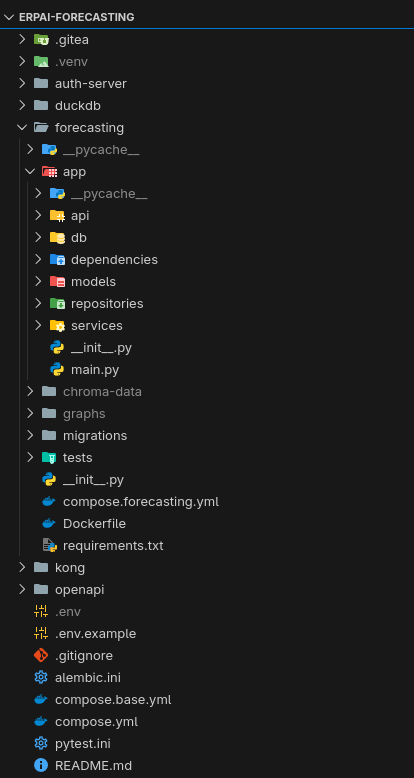
\includegraphics[width=0.6\linewidth]{img/repository.png}
    \caption{Struttura delle directory del progetto.}
    \label{fig:repo-structure}
\end{figure}

\newpage
